\clearpage

\def\chaptertitle{Background}

\lhead{\emph{\chaptertitle}}

\chapter{\chaptertitle}
\label{ch:background}

In this chapter, a brief overview of microservice architectures is provided in section \ref{sec:micro-svc-arc}. This includes a brief description of the architecture of Kubernetes, along with its scheduling and autoscaling algorithms. Finally, section \ref{sec:lit-review} comprises of a detailed literature review of the state-of-the-art autoscaling algorithms and a comparison of their performances and drawbacks.

\section{Microservice Architecture}
\label{sec:micro-svc-arc}

Microservice architectures involve decomposing an application into several loosely coupled services, and deploying them on separate servers known as ``nodes''. These services communicate with each other through a lightweight framework such as RESTful APIs \cite{li2021understanding}. Within these services, application data and commands are stored and executed within ``containers''. Typically, these architectures provide scalability, as well as ease of deployment and modification. Availability however, remains an important concern for such deployments. For a deployment to be classified as ``highly available'', it must be accessible at least 99.999\% of the time. For example, a highly available search engine would only face 5 minutes of down time per year \cite{nabi2016availability}. Therefore, an orchestration mechanism is required to manage the deployment and communication of these containers.\par

\begin{figure}[htb]
    \centering
    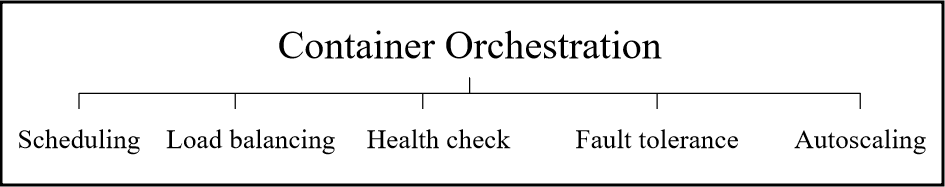
\includegraphics[width=0.9\linewidth]{Figures/Container-Orchestration.png}
    \caption{Features of Container Orchestration}
    \label{fig:container-orchestration}
\end{figure}

Container orchestration allows the microservice application to customize how the deployment, monitoring, and controlling functions \cite{casalicchio2019container}. Figure \ref{fig:container-orchestration} depicts the typical features of container orchestration.\par
\textit{Scheduling} defines the rules on the number of containers to be executed at any given time. Scheduling also places containers on specific nodes based on availability and best performance.\par
\textit{Load balancing} distributes the resource usage among multiple microservice nodes. By default, a round-robin policy is implemented, although more complex policies may be implemented at the discretion of the developer.\par
\textit{Health checks} ensure that the container is still capable of responding to queries. Typically, these are done using a periodic light-weight HTTP request and verifying the response.\par
\textit{Fault tolerance} maintains several replicas of containers, a strategy commonly used to achieve the high availability mentioned above. Health checks are used to ensure the replicas are functioning, and they typically have strategies to ensure there is no mismatch in data between two fault tolerant containers.\par
\textit{Autoscaling} is the process of automatically adding or removing resources or containers. Internal metrics such as CPU usage are typically used, however custom policies can also be implemented at the discretion of the developer.\par

\subsection{Kubernetes Architecture}
\label{subsec:k8s-overview}

Kubernetes \footnote{\url{https://kubernetes.io/}} is one of the most popular open-source container orchestration platforms \cite{vayghan2019kubernetes}. Initially referred to as ``Borg'', the project was used internally at Google to deploy the majority of their cloud applications before becoming an open-source application \cite{burns2016borg}. Figure \ref{fig:k8s-arch} shows the high-level architecture. The Kubernetes deployment has a controller / worker architecture. The nodes in the Kubernetes cluster are split into either \textit{control plane nodes} and \textit{data plane nodes}. The \textit{control plane nodes} have a collection of processes which help monitor and maintain the desired state of the deployment. The \textit{data plane nodes} contain processes which run the containers doing the actual work, and are managed by the control plane.\par
The smallest unit of work in a Kubernetes deployment is known as a \textit{pod} \cite{baier2017getting}. This is a collection of containers sharing an IP address and port. In summary, microservice architectures are said to be containerized and deployed on Kubernetes in the form of pods \cite{vayghan2019kubernetes}.\par
\begin{figure}[htb]
    \centering
    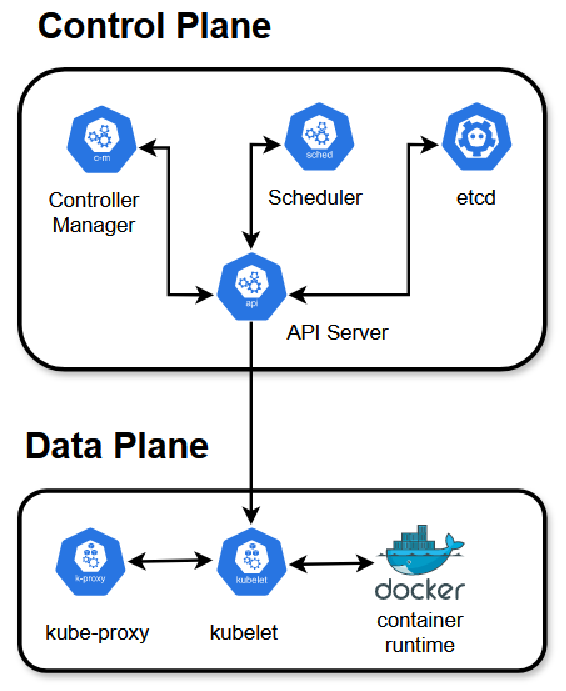
\includegraphics[width=0.5\linewidth]{Figures/K8s-Architecture.pdf}
    \caption{Kubernetes Architecture}
    \label{fig:k8s-arch}
\end{figure}

\subsubsection{Data Plane}
\label{subsubsec:k8s-data-plane}

The \textit{container runtime} is a process which downloads or ``pulls'' the image for the required container onto the node. Kubernetes supports a wide range of runtimes, but some of the popular solutions are CRI-O \footnote{\url{https://cri-o.io/}}, containerd \footnote{\url{https://containerd.io/}}, and Docker \footnote{\url{https://www.docker.com/}}.\par

The most important process running on every data plane node is the \textit{kubelet}. This process executes the image assigned to the node via the container runtime, perform health checks, and reports the node status to the control plane.\par

Another data plane process is the \textit{kube-proxy}, which manages the rules for forwarding requests to services, as well as the IP tables of nodes. If a service is added or removed, kube-poxy updates the IP table accordingly.\par

\subsubsection{Control Plane}
\label{subsubsec:k8s-control-plane}
The \textit{API Server} is the primary communication endpoint for the entire deployment. Every component in the architecture communicates through it to exchange information. It is also used to update the current deployment state. The API Server is a simple RESTful API implementation, exposing well-documented APIs for access by other components as well as developers. Multiple replicas of this component are typically maintained to ensure high availability.\par

The \textit{etcd} is a data store which persists the deployment state in a key-value format. The data is serialized unlike in the stateless API server. This data adheres the properties of \textit{recovery} and \textit{availability}. \textit{Recovery} ensures that any corruption of data is reverted using a system of backups such as checkpoints. \textit{Availability} ensures that the deployment is reachable by the end-user regardless of the traffic being requested on the network.\par

\textit{Controller Manager} implements the desired deployment state. During initial deployment, the controller manager inputs the required workload as the desired state, after which it continually monitors the deployment state using a system of looping controls. If the deployment requires modifications, they are achieved using the API server, and the deployment is brought back into alignment with the desired state.\par

Finally, the \textit{scheduler} decides the location where the pod will be deployed. The scheduler runs a control loop which searches for uncheduled pods using the API server. It then assigns the pods to a dataplane node based on several predicates and priorities such as resource requirements and node affinity respectively.

\section{Autoscaling Overview}
\label{sec:autoscaling}

Apart from intelligently scheduling pods to data plane nodes \cite{kayal2020kubernetes}, Kubernetes has the provisions to dynamically respond to changes in resource requirements. This process of scaling nodes, pods, or other resources depending on requirements in an automated manner is known as \textit{autoscaling}. Kubernetes supports three variations of autoscaling.\par

\textit{Cluster autoscaling} modifies the number of nodes running in the entire deployment, or cluster. Dynamically allocating nodes based on resource requirements helps to manage the cost of running Kubernetes deployments on external platforms such as Amazon \footnote{\url{https://docs.aws.amazon.com/eks/}} or Google \footnote{\url{https://cloud.google.com/kubernetes-engine/}}. The autoscaler works by looping through two tasks. The first watches for unscheduled pods, the second checks if the current deployed pods (pods which are running on the data plane) can be merged on a smaller number of nodes.\par

\textit{Vertical pod autoscaling} modifies the CPU and memory resources assigned to pods. By default, the scheduler reserves a larger amount of these resources to pods than is usually required. By performing vertical pod autoscaling, the cluster can better manage its over-provisioned resources in real-time.\par

\textit{Horizontal pod autoscaling} is the most commonly used autoscaling strategy \cite{baresi2021kosmos}, it modifies the number of pods assigned to a task, based on the resources being requested. Kubernetes implements this using a periodic control loop which runs every 15 seconds by default. The control manager compares the actual resource utilization with the target utilization defined by the deployment script, and scales the number of pods accordingly.

\subsection{Custom Autoscaling}
\label{subsec:custom-autoscaling}

The default horizontal pod autoscaler uses pod CPU and memory utilization when making its scaling decisions. However, these metrics may be too rigid when it comes to edge architectures \cite{coulson2020adaptive}. The strict SLA constraints in place, along with the lower amount of resources present in the edge layer as compared to the cloud layer, make it imperative for custom metrics to be employed to autoscale resources as efficiently as possible.\par

Figure \ref{fig:custom-autoscale-overview} depicts the general architecture of the custom autoscaler. Typically, the autoscaler queries metrics from the default metrics registry, which acts as a central store for all metrics that are exposed to the developer. Three interfaces to this registry are exposed:
\begin{itemize}
    \item \textit{Resource metric API} is used to access predefined metrics such as CPU and memory resources of both pods as well as nodes.
    \item \textit{Custom metric API} contains user-defined custom metrics associated with all Kubernetes objects.
    \item \textit{External metrics API} contains metrics of objects which are not associated with Kubernetes.
\end{itemize}
For custom metric autoscaling, the autoscaler must be configured in a way where the metrics can be fetched from the custom metric API. This is done by configuring the custom metric server, several frameworks to simplify this process such as the Kubernetes Instrumentation SIG \footnote{\url{https://github.com/kubernetes/community/tree/master/sig-instrumentation}} exist which simplify the server building process.

\begin{figure}[htb]
    \centering
    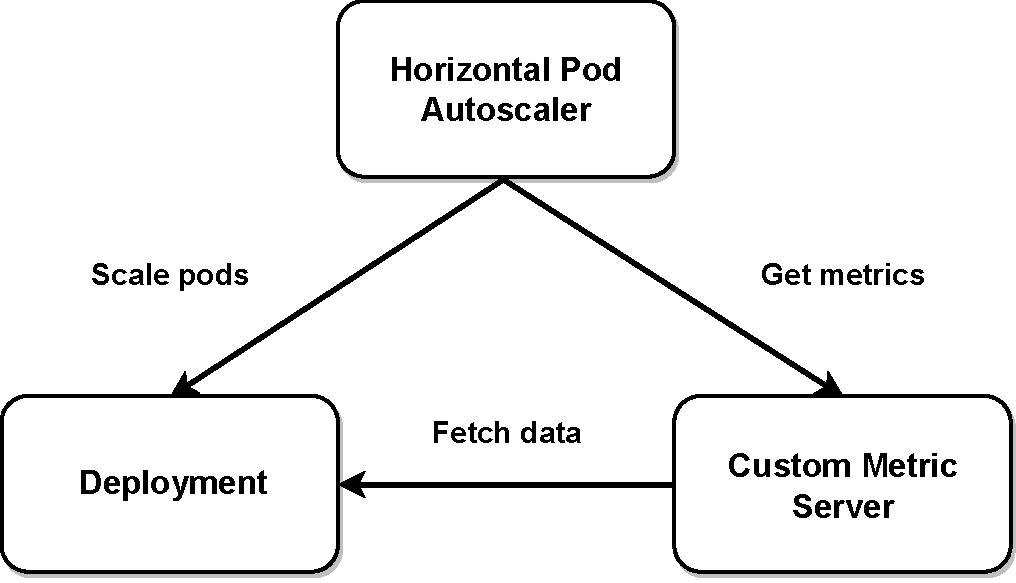
\includegraphics[width=.5\linewidth]{Figures/Custom-Metrics-Autoscaling.pdf}
    \caption{Custom Autoscaler Architecture Overview.}
    \label{fig:custom-autoscale-overview}
\end{figure}

\section{Literature Review}
\label{sec:lit-review}